\documentclass[psamsfonts]{amsart}
\usepackage[utf8]{inputenc}
\usepackage{amsfonts}
\usepackage[hidelinks]{hyperref}
\hypersetup{
pdftitle={Deep computations and NIP}
pdfsubject={Mathematics, Set Theory},
pdfauthor={Luciano Salvetti, Tonatiuh Matos-Wiederhold},
pdfkeywords={}
}
\usepackage{amsmath}
\usepackage{xcolor}
\usepackage{amsthm}
\usepackage{pdflscape}
\usepackage{pgfplots}
\usepackage{mathrsfs}
\usepackage{enumitem}
\usepackage{euler}
\usepackage{tikz}
\usetikzlibrary{trees}

\newtheorem{thm}{Theorem}[section]
\newtheorem{cor}[thm]{Corollary}
\newtheorem{prop}[thm]{Proposition}
\newtheorem{lem}[thm]{Lemma}
\newtheorem{conj}[thm]{Conjecture}
\newtheorem{quest}[thm]{Question}
\newtheorem*{claim}{Claim}
\newtheorem{fact}[thm]{Fact}
\newtheorem{ppty}[thm]{Property}

\theoremstyle{definition}
\newtheorem{defn}[thm]{Definition}
\newtheorem{question}[thm]{Question}
\newtheorem{defns}[thm]{Definitions}
\newtheorem{con}[thm]{Construction}
\newtheorem{exmp}[thm]{Example}
\newtheorem{exmps}[thm]{Examples}
\newtheorem{notn}[thm]{Notation}
\newtheorem{notns}[thm]{Notations}
\newtheorem{addm}[thm]{Addendum}
\newtheorem{exer}[thm]{Exercise}
\newtheorem{limit}[thm]{Limitation}

\theoremstyle{remark}
\newtheorem{rem}[thm]{Remark}
\newtheorem{rems}[thm]{Remarks}
\newtheorem{warn}[thm]{Warning}
\newtheorem{sch}[thm]{Scholium}

\makeatletter
\let\c@equation\c@thm
\makeatother
\numberwithin{equation}{section}

%\bibliographystyle{plain}

%--------Meta Data: Fill in your info------
\title{Deep computations and NIP}

\author[Dueñez, Iovino, Matos-Wiederhold, Salvetti, Tall]{
Eduardo Dueñez$^{1}$ \qquad
José Iovino$^{1}$ \qquad
Tonatiuh Matos-Wiederhold$^{2}$ \qquad
Luciano Salvetti$^{2}$ \qquad
Franklin D. Tall$^{2}$
}

\usepackage{lineno}
\linenumbers

\begin{document}

\maketitle

{\centering\tiny\vspace{-0.6cm}
$^{1}$Department of Mathematics, University of Texas at San Antonio\\
$^{2}$Department of Mathematics, University of Toronto\\
}

\begin{abstract}
This paper revisits and extends a bridge between functional analysis and model theory, emphasizing its relevance to the theoretical foundations of machine learning. We show that the compactness behavior of families of Baire class 1 functions mirrors the learnability conditions in the sense of \emph{Probably Approximately Correct} (PAC) learning, and that the failure of compactness corresponds to the presence of infinite \emph{Vapnik-Chervonenkis} (VC) dimension. From this perspective, Rosenthal compacta emerge as the natural topological counterpart of PAC-learnable concept classes, while NIP vs. IP structures capture the precise boundary between analytical regularity and combinatorial intractability. These parallels suggest a unified framework linking compactness, definability, and learnability, exemplifying how the topology of function spaces encodes the algorithmic and epistemic limits of prediction.
\end{abstract}

\maketitle

\section{Introduction}

Suppose that $A$ is a subset of the real line $\mathbb R$ and that $\overline A$ is its \emph{closure}. It is a well-known fact that any point of closure of $A$, say $x\in\overline A$, can be \emph{approximated} by points inside of $A$, in the sense that a sequence $\{x_n\}_{n\in\mathbb N}\subseteq A$ must exist with the property that $\lim_{n\to\infty}x_n=x$. For most applications we wish to approximate objects more complicated than points, such as functions.

Suppose we wish to build a neural network that decides, given an 8 by 8 black-and-white image of a hand-written scribble, what single decimal digit the scribble represents. Maybe there exists $f$, a function representing an optimal solution to this classifier. Thus if $X$ is the set of all (possible) images, then for $I\in X$, $f(I)\in\{0,1,2,\dots,9\}$ is the ``best'' (or ``good enough'' for whatever deployment is needed) possible guess. Training the neural network involves approximating $f$ until its guesses are within an acceptable error range. In general, $f$ might be a function defined on a more complicated topological space $X$.

Often computers' viable operations are restricted (addition, subtraction, multiplication, division, etc.) and so we want to approximate a complicated function using simple functions (like polynomials). The problem is that, in contrast with mere points, functions in the closure of a set of functions need not be approximable (meaning the pointwise limit of a sequence of functions) by functions in the set.

Functions that are the pointwise limit of continuous functions are \emph{Baire class 1 functions}, and the set of all of these is denoted by $B_1(X)$. Notice that these are not necessarily continuous themselves! A set of Baire class 1 functions, $A$, will be relatively compact if its closure consists of just Baire class 1 functions (we delay the formal definition of \emph{relatively compact} until Section~\ref{sec:prelim}, but the fact mentioned here is sufficient). The Bourgain-Fremlin-Talagrand (BFT) theorem reveals a precise correspondence between relative compactness in $B_1(X)$ and the model-theoretic notion of \emph{Non-Independence Property} (NIP). This was realized by Pierre Simon in \cite{Simon_2015_RosenthalNIP}. 

Simon's insight was to view definable families of functions as sets of real-valued functions on type spaces and to interpret relative compactness in $B_1(X)$ as a form of ``tame behavior'' under ultrafilter limits. From this perspective, NIP theories are those whose definable families behave like relatively compact sets of Baire class 1 functions, avoiding the wild, $\beta\mathbb N$-like configurations that witness unstability. This observation opened a new bridge between analysis and logic: topological compactness corresponds to the absence of combinatorial independence. Simon's later developments connected these ideas to \emph{Keisler measures} and \emph{empirical averages}, allowing tools from functional analysis to be used to study learnability and definable types. This reinterpretation of model-theoretic tameness through the lens of the BFT theorem has made NIP a central notion not only in stability theory but also in contemporary connections with learning theory and ergodic analysis.

Historically, the notion of NIP arises from Shelah's foundational work on the classification theory of models. In his seminal book \emph{Unstable Theories}~\cite{shelah1978unstable}, Shelah introduced the independence property as a key dividing line within unstable structures, identifying the class of stable theories inside those in which this property fails. Fix a first-order formula $\varphi(x,y)$ in a language $L$ and a model $M$ of an $L$-theory $T$. We say that $\varphi(x,y)$ has the \emph{independence property (IP)} in $M$ if there is a sequence $(c_i)_{i\in\mathbb N}\subseteq M^{|x|}$ such that for every $S\subseteq\mathbb N$ there is $a_S\in M^{|y|}$ with $$\forall i\in\mathbb N,\qquad M\models\varphi(c_i,a_S)\quad\iff\quad i\in S.$$ The formula $\phi(x,y)$ has the IP if it does so in some model $M$, and the formula has the \emph{non-independence property (NIP)} if it does not have the IP. The latter notion of NIP generalizes stability by forbidding the full combinatorial independence pattern while allowing certain controlled forms of unstability. Thus, Simon's interpretation of the BFT theorem can be viewed as placing Shelah's dividing line into a topological-analytic framework, connecting the earliest notions of stability to compactness phenomena in spaces of Baire class 1 functions.

One of the most important innovations in Machine Learning is the mathematical notion, introduced by Turing Awardee Leslie Valiant in the 1980s, of ‘probably approximately correct learning’, or PAC-learning for short~\cite{bendavid2019understanding}. We give a standard but short overview of these concepts in the context that is relevant to this work.

Consider the following important idea in data classification. Suppose that $A$ is a set and that $\mathcal C$ is a collection of sets. We say that $\mathcal C$ \emph{shatters} $A$ if every subset of $A$ is of the form $C\cap A$ for some $C\in\mathcal C$. For a classical geometric example, if $A$ is the set of four points on the Euclidean plane of the form $(\pm1,\pm1)$, then the collection of all half-planes does not shatter $A$, the collection of all open balls does not shatter $A$, but the collection of all convex sets shatters $A$. While $A$ need not be finite, it will usually be assumed to be so in Machine Learning applications. A finer way to distinguish collections of sets that shatter a given set from those that do not is by the \emph{Vapnik-Chervonenkis dimension (VC-dimension)}, which is equal to the cardinality of the largest finite set shattered by the collection, in case it exists, or to infinity otherwise.

A concrete illustration of these ideas appears when considering threshold classifiers on the real line. Let $\mathcal{H}$ be the collection of all indicator functions $h_t$ given by $h_t(x)=1$ if $x\leq t$ and $h_t(x)=0$ otherwise. Each $h_t$ is a Baire class 1 function, and the family $\mathcal{H}$ is relatively compact in $B_1(\mathbb{R})$. In model-theoretic terms, $\mathcal{H}$ is NIP, since no configuration of points and thresholds can realize the full independence pattern of a binary matrix. By contrast, the family of parity functions $\{x\mapsto (-1)^{\langle w,x\rangle}:w\in\{0,1\}^n\}$ on $\{0,1\}^n$ (here ${\langle w,x\rangle}$ is the usual vector dot product) has the independence property and fails relative compactness in $B_1(X)$, capturing the analytical meaning of instability. This dichotomy mirrors the behavior of concept classes with finite versus infinite VC dimension in statistical learning theory.

Going back to the model theoretic framework, let $$\mathcal F_\varphi(M):=\{\varphi(M,a):a\in M^{|y|}\}$$ be the family of subsets of $M^{|x|}$ defined by instances of the formula $\varphi$, where $\varphi(M,a)$ is the set of $|x|$-tuples $c$ in $M$ for which $M\models \varphi(c,a)$. The fundamental theorem of statistical learning states that a binary hypothesis class is PAC-learnable if and only if it has finite VC-dimension, and the subsequent theorem connects the rest of the concepts presented in this section.

\begin{thm}[Laskowski]
    The formula $\varphi(x,y)$ has the NIP if and only if $\mathcal F_\varphi(M)$ has finite VC-dimension.
\end{thm}

For two simple examples of formulas satisfying the NIP, consider first the language $L=\{<\}$ and the model $M=(\mathbb R,<)$ of the reals with their usual linear order. Take the formula $\varphi(x,y)$ to mean $x<y$, then $\varphi(M,a)=(-\infty,a)$, and so $\mathcal F_\varphi(M)$ is just the set of left open rays. The VC-dimension of this collection is 1, since it can shatter a single point, but no two point set can be shattered since the rays are downwards closed. Now in contrast, the collection of open intervals, given by the formula $\varphi(x;y_1,y_2):=(y_1<x)\land(x<y_2)$, has VC-dimension 2.

In this work, we study the corresponding notions of NIP (and hence PAC-learnability) in the context of Compositional Computation Structures introduced in \cite{alva2024approximability}.

\section{General topological preliminaries}\label{sec:prelim}

In this section we give preliminaries from general topology and function space theory. We include some of the proofs for completeness but a reader familiar with these topics may skip them.

A \emph{Polish space} is a separable and completely metrizable topological space. The most important examples are the reals $\mathbb R$, the Cantor space $2^\mathbb N$ (the set of all infinite binary sequences, endowed with the product topology), and the Baire space $\mathbb N^\mathbb N$ (the set of all infinite sequences of naturals, also with the product topology). Countable products of Polish spaces are Polish; this includes spaces like $\mathbb R^\mathbb N$, the space of sequences of real numbers. A subspace of a Polish space is itself Polish if and only if it is a $G_\delta$-set, that is, it can be written as the intersection of a countable family of open subsets; in particular, closed subsets and open subsets of Polish spaces are also Polish spaces.

In this work we talk a lot about subspaces, and so there is a pertinent subtlety of the definitions worth mentioning: \emph{completely metrizable space} is not the same as \emph{complete metric space}; for an illustrative example, notice that $(0,1)$ is homeomorphic to the real line, and thus a Polish space (being Polish is a topological property), but with the metric inherited from the reals, as a subspace, $(0,1)$ is \textbf{not} a complete metric space. In summary, a Polish space has its topology generated by \emph{some} complete metric, but other metrics generating the same topology might not be. In practice, such as when studying descriptive set theory, one finds that we can often keep the metric implicit.

Given two topological spaces $X$ and $Y$ we denote by $B_1(X,Y)$ the set of all functions $f:X\to Y$ such that for all open $U\subseteq Y$, $f^{-1}[U]$ is an $F_\sigma$ subset of $X$ (that is, a countable union of closed sets); we call these types of functions \emph{Baire class 1 functions}. When $Y=\mathbb{R}$ we simply denote this collection by $B_1(X)$. We endow $B_1(X,Y)$ with the topology of pointwise convergence (the topology inherited from the product topology of $Y^X$). By $C_p(X,Y)$ we denote the set of all continuous functions $f:X\rightarrow Y$ with the topology of pointwise convergence. Similarly, $C_p(X):=C_p(X,\mathbb{R})$. A natural question is, how do topological properties of $X$ translate to $C_p(X)$ and vice versa? These questions, and in general the study of these spaces, are the concern of $C_p$-theory, an active field of research in general topology which was pioneered by A. V. Arhangel’skiĭ and his students in the 1970's and 1980's. This field has found many exciting applications in model theory and functional analysis (see \cite{iovino2020banach}). Good recent surveys on the topics include \cite{hamel2023cp} and \cite{tkachuk2011cp}. We begin with the following:

\begin{fact}
If $X$ is metrizable, then $C_p(X,Y)\subseteq B_1(X,Y)$.
\end{fact}

The proof of the following fact (due to Baire) can be found in Section 10 of \cite{Todorcevic_1997_TopicsTop}.

\begin{fact}[Baire]\label{baire}
    If $X$ is a complete metric space, then the following are equivalent:
    \begin{itemize}
        \item [(i)] $f$ is a Baire class 1 function, that is, $f\in B_1(X)$.
        \item [(ii)] $f$ is a pointwise limit of continuous functions.
        \item [(iii)] For every closed $F\subseteq X$, the restriction $f|_F$ has a point of continuity.
    \end{itemize}
    Moreover, if $X$ is Polish and $f\notin B_1(X)$, then there exists countable $D_0,D_1\subseteq X$ and reals $a<b$ such that $\overline{D_0}=\overline{D_1}$, $D_0\subseteq f^{-1}(-\infty,a]$ and $D_1\subseteq f^{-1}[b,\infty)$.
\end{fact}

A subset $L\subseteq X$ is \emph{relatively compact} in $X$ if the closure of $L$ in $X$ is compact. Relatively compact subsets of $B_1(X)$ (for $X$ Polish space) have been objects of interest to many people working in Analysis and Topological Dynamics. We begin with the following well-known result. Recall that a set $A\subseteq\mathbb{R}^X$ of real-valued functions is \emph{pointwise bounded} if for every $x\in X$ there is $M_x>0$ such that $|f(x)|<M_x$ for all $f\in A$. We include the proof for the reader's convenience:

\begin{lem}
    Let $X$ be a Polish space and $A\subseteq B_1(X)$ be pointwise bounded. The following are equivalent:
    \begin{itemize}
        \item [(i)] $A$ is relatively compact in $B_1(X)$.
        \item [(ii)] $A$ is relatively countably compact in $B_1(X)$, i.e., every countable subset of $A$ has an accumulation point in $B_1(X)$.
        \item [(iii)] $\overline{A}\subseteq B_1(X)$, where $\overline{A}$ denotes the closure in $\mathbb{R}^X$.
    \end{itemize}
\end{lem}

\begin{proof}
    By definition, being pointwise bounded means that there is, for each $x\in X$, $M_x>0$ such that, for every $f\in A$, $|f(x)|\leq M_x$.

    (i)$\Rightarrow$(ii) holds in general. 

    (ii)$\Rightarrow$(iii) Assume that $A$ is relatively countably compact in $B_1(X)$ and that $f\in\overline A\setminus B_1(X)$. By Fact \ref{baire}, there are countable $D_0,D_1\subseteq X$ with $\overline {D_0}=\overline{D_1}$, and $a<b$ such that $D_0\subseteq f^{-1}(-\infty,a]$ and $D_1\subseteq f^{-1}[b,\infty)$. We claim that there is a sequence $\{f_n\}_{n\in\mathbb N}\subseteq A$ such that for all $x\in D_0\cup D_1$, $\lim_{n\to\infty}f_n(x)=f(x)$. Indeed, use the countability to enumerate $D_0\cup D_1$ as $\{x_n\}_{n\in\mathbb N}$. Then find, for each positive $n$, $f_n\in A$ with $|f_n(x_i)-f(x_i)|<\frac1n$ for all $i\leq n$. The claim follows.

    By relative countable compactness of $A$, there is an accumulation point $g\in B_1(X)$ of $\{f_n\}_{n\in\mathbb N}$. It is straightforward to show that since $f$ and $g$ agree on $D_0\cup D_1$, $g$ does not have a point of continuity on the closed set $\overline{D_0}=\overline{D_1}$, which contradicts Fact~\ref{baire}.

    (iii)$\Rightarrow$(i) Suppose that $\overline A\subseteq B_1(X)$. Then $\overline{A}\cap B_1(X)=\overline A$ is a closed subset of $\prod_{x\in X}[-M_x,M_x]$; Tychonoff's theorem states that the product of compact spaces is always compact, and since closed subsets of compact spaces are compact, $\overline A$ must be compact, as desired.
\end{proof}

\subsection{From Rosenthal's dichotomy to NIP}

The fundamental idea that connects the rich theory here presented to real-valued computations is the concept of an \emph{approximation}. In the reals, points of closure from some subset can always be approximated by points inside the set, via a convergent sequence. For more complicated spaces, such as $C_p(X)$, this fails in a remarkably intriguing way. Let us show an example that is actually the protagonist of a celebrated result. Consider the Cantor space $X=2^\mathbb N$ and let $p_n(x)=x(n)$ define a continuous mapping $X\to\{0,1\}$. Then one can show (see Chapter~1.1 of \cite{Todorcevic_1997_TopicsTop} for details) that, perhaps surprisingly, the only continuous functions in the closure of $\{p_n\}_{n\in\mathbb N}$ are the functions $p_n$ themselves; moreover, none of the subsequences of $\{p_n\}_{n\in\mathbb N}$ converge. In some sense, this example is the worst possible scenario for convergence. The topological space obtained from this closure is well-known. Topologists refer to it as the Stone-Čech compactification of the discrete space of natural numbers, or $\beta\mathbb N$ for short, and it is an important object of study in general topology.

\begin{thm}[Rosenthal's Dichotomy]
    If $X$ is Polish and $\{f_n\}\subseteq C_p(X)$ is pointwise bounded, then either $\{f_n\}_{n\in\mathbb N}$ contains a convergent subsequence or a subsequence whose closure (in $\mathbb R^X$) is homeomorphic to $\beta\mathbb N$.
\end{thm}

In other words, a pointwise bounded set of continuous functions will either contain a subsequence that converges or a subsequence whose closure is essentially the same as the example mentioned in the previous paragraphs (the worst possible scenario). Note that in the preceding example, the functions are trivially pointwise bounded in $\mathbb R^X$ as the functions can only take values $0$ and $1$.

If we intend to generalize our results from $C_p(X)$ to the bigger space $B_1(X)$, we find a similar dichotomy. Either every point of closure of the set of functions will be a Baire class 1 function, or there is a sequence inside the set that behaves in the worst possible way (which in this context, is the IP!). The theorem is usually not phrased as a dichotomy but rather as an equivalence (with the NIP instead):

\begin{thm}[Bourgain-Fremlin-Talagrand, Theorem 4G in \cite{BFT_1978_PCompactBaire}]\label{BFT}
    Let $X$ be a Polish space and $A\subseteq C_p(X)$ be pointwise bounded. The following are equivalent:
    \begin{itemize}
        \item [(i)] $A$ is relatively compact in $B_1(X)$, i.e., $\overline{A}\subseteq B_1(X)$.
        \item [(ii)] For every $\{f_n\}_{n\in\mathbb N}\subseteq A$ and for every $a<b$ there is $I\subseteq\mathbb{N}$ such that
$$\bigcap_{n\in I}f_n^{-1}(-\infty,a]\cap\bigcap_{n\notin I}f_n^{-1}[b,\infty)=\emptyset.$$
    \end{itemize}
\end{thm}

Our goal now is to characterize relatively compact subsets of $B_1(X,Y)$ when $Y=\mathbb{R}^\mathcal{P}$ with $\mathcal{P}$ countable. Given $P\in\mathcal{P}$ we denote the \emph{projection map} onto the $P$-coordinate by $\pi_P:\mathbb{R}^\mathcal{P}\rightarrow\mathbb{R}$. From a high-level topological interpretation, the subsequent lemma states that, in this context, the spaces $\mathbb R$ and $\mathbb R^\mathcal P$ are really not that different, and that if we understand the Baire class 1 functions of one space, then we also understand the functions of both. In fact, $\mathbb R$ and any other Polish space is embeddable as a closed subspace of $\mathbb R^\mathcal P$.

\begin{lem}\label{baire 1 and projections}
    Let $X$ be a Polish space and $\mathcal{P}$ be a countable set. Then, $f\in B_1(X,\mathbb{R}^\mathcal{P})$ if and only if $\pi_P\circ f\in B_1(X)$ for all $P\in\mathcal{P}$.
\end{lem}

\begin{proof}
    Only one implication needs a proof. Suppose that $\pi_P\circ f\in B_1(X)$ for all $P\in\mathcal{P}$. Let $V$ be a basic open subset of $\mathbb{R}^\mathcal{P}$. That is, there exists a finite $\mathcal{P}'\subseteq\mathcal{P}$ such that $V=\bigcap_{P\in\mathcal{P}'}\pi_P^{-1}[U_P]$ where $U_P$ is open in $\mathbb{R}$. Finally, 
    $$f^{-1}[V]=\bigcap_{P\in\mathcal{P}'}(\pi_P\circ f)^{-1}[U_P]$$ is an $F_\sigma$ set. Since $\mathcal{P}$ is countable, $\mathbb{R}^\mathcal{P}$ is second countable so every open set $U$ in $\mathbb{R}^\mathcal{P}$ is a countable union of basic open sets. Hence, $f^{-1}[U]$ is $F_\sigma$.
\end{proof}

Below we consider $\mathcal P$ with the discrete topology. For each $f:X\rightarrow\mathbb{R}^\mathcal{P}$ denote $\hat f(P,x):=\pi_P\circ f(x)$ for all $(P,x)\in\mathcal{P}\times X$. Similarly, for each $g:\mathcal{P}\times X\rightarrow\mathbb{R}$ denote $\check g(x)(P):=g(P,x)$. Given $A\subseteq (\mathbb{R}^\mathcal{P})^X$, we denote $\hat A$ as the set of all $\hat f$ such that $f\in A$.

The map $\left(\mathbb R^\mathcal P\right)^X\to\mathbb R^{\mathcal P\times X}$ given by $f\mapsto\hat f$ is a homeomorphism and its inverse is given by $g\mapsto\check g$.

\begin{lem}\label{homeo}
    Let $X$ be a Polish space and $\mathcal{P}$ be countable. Then, $f\in B_1(X,\mathbb R^\mathcal P)$ if and only if $\hat f\in B_1(\mathcal P\times X)$.
\end{lem}

\begin{proof}
    ($\Rightarrow$) Given an open set of reals $U$, we have that for every $P\in\mathcal P$, $f^{-1}[\pi_P^{-1}[U]]$ is $F_\sigma$ by Lemma~\ref{baire 1 and projections}. Given that $\mathcal P$ is a discrete countable space, we observe that
    $$\hat f^{-1}[U]=\bigcup_{P\in\mathcal P}\left(\{P\}\times f^{-1}[\pi_P^{-1}[U]]\right)
    $$ is also an $F_\sigma$ set.
    ($\Leftarrow$) By lemma \ref{baire 1 and projections} it suffices to show that $\pi_P\circ f\in B_1(X)$ for all $P\in\mathcal{P}$. Fix an open $U\subseteq\mathbb{R}$. Write $\hat{f}^{-1}[U]=\bigcup_{n\in\mathbb{N}}F_n$ where $F_n$ is closed in $\mathcal{P}\times X$. Then,
    $$(\pi_P\circ f)^{-1}[U]=\bigcup_{n\in\mathbb{N}}\{x\in X:(P,x)\in F_n\}$$
    which is $F_\sigma$.
\end{proof}

We now direct our attention to a notion of the NIP that is more general than the one from the introduction. It can be interpreted as a sort of continuous version of the one presented in the preceding section.

\begin{defn}
    We say that $A\subseteq \mathbb{R}^X$ has the \emph{Non-Independence Property} (NIP) if and only if for every $\{f_n\}_{n\in\mathbb N}\subseteq A$ and for every $a<b$ there are finite disjoint sets $E,F\subseteq\mathbb{N}$ such that
    $$\bigcap_{n\in E}f_n^{-1}(-\infty,a]\cap\bigcap_{n\in F}f_n^{-1}[b,\infty)=\emptyset.$$
\end{defn}

Note that if $X$ is compact and $A\subseteq C_p(X)$, then $A$ has the NIP if and only if for every $\{f_n\}_{n\in\mathbb N}\subseteq A$ and for every $a<b$ there is $I\subseteq\mathbb{N}$ such that
$$\bigcap_{n\in I}f_n^{-1}(-\infty,a]\cap\bigcap_{n\notin I}f_n^{-1}[b,\infty)=\emptyset.$$

Given $A\subseteq Y^X$ and $K\subseteq X$ we write $A|_K:=\{f|_K:f\in A\}$, i.e., the set of all restrictions of functions in $A$ to $K$. The following Theorem is a slightly more general version of Theorem \ref{BFT}.

\begin{thm}\label{Generalized BFT}
    Assume that $\mathcal P$ is countable, $X$ is a Polish space, and $A\subseteq C_p(X,\mathbb R^\mathcal P)$ be such that $\pi_P\circ A$ is pointwise bounded for all $P\in\mathcal{P}$. The following are equivalent for every compact $K\subseteq X$:

    \begin{enumerate}
        \item $\overline{A|_K}\subseteq B_1(K,\mathbb R^\mathcal P)$.
        \item $\pi_P\circ A|_K$ has the NIP for every $P\in\mathcal P$.
    \end{enumerate}
\end{thm}

\begin{proof}
    (1)$\Rightarrow$(2). Let $P\in\mathcal{P}$. Fix $\{f_n\}_{n\in\mathbb N}\subseteq A$ and $a<b$. By (1) we have that $\overline{A|_K}\subseteq B_1(K,\mathbb{R}^\mathcal{P})$. Applying the homeomorphism $f\mapsto \hat{f}$ and using lemma \ref{homeo} we get $\overline{\hat{A}|_{\mathcal{P}\times K}}\subseteq B_1(\mathcal{P}\times K)$. By Theorem \ref{BFT}, there is $I\subseteq\mathbb{N}$ such that
    $$(\mathcal{P}\times K)\cap\bigcap_{n\in I}\hat{f_n}^{-1}(-\infty,a]\cap\bigcap_{n\notin I}\hat{f_n}^{-1}[b,\infty)=\emptyset$$
    Hence,
    $$K\cap\bigcap_{n\in I}(\pi_P\circ f_n)^{-1}(-\infty,a]\cap\bigcap_{n\notin I}(\pi_P\circ f_n)^{-1}[b,\infty)=\emptyset$$
    By compactness, there are finite $E\subseteq I$ and $F\subseteq\mathbb{N}\backslash I$ such that
    $$K\cap\bigcap_{n\in E}(\pi_P\circ f_n)^{-1}(-\infty,a]\cap\bigcap_{n\in F}(\pi_P\circ f_n)^{-1}[b,\infty)=\emptyset$$
    Thus, $\pi_P\circ A|_L$ has the NIP.

    (2)$\Rightarrow$(1) Fix $f\in\overline{A|_K}$. By lemma \ref{baire 1 and projections} it suffices to show that $\pi_P\circ f\in B_1(K)$ for all $P\in\mathcal{P}$. By (2), $\pi_P\circ A|_K$ has the NIP. Hence, by Theorem \ref{BFT} we have $\overline{\pi_P\circ A|_K}\subseteq B_1(K)$. But then $\pi_P\circ f\in\overline{\pi_P\circ A|_K}\subseteq B_1(K)$.
\end{proof}

Lastly, a simple but significant result that helps understand the operation of restricting a set of functions to a specific subspace of the domain space $X$, of course in the context of the NIP, is that we may always assume that said subspace is closed. Concretely, whether we take its closure or not has no effect on the NIP:

\begin{lem}\label{NIP and closure}
    Assume that $X$ is Hausdorff and that $A\subseteq C_p(X)$. The following are equivalent for every $L\subseteq X$:
    \begin{itemize}
        \item [(i)] $A_L$ has the NIP.
        \item [(ii)] $A|_{\overline{L}}$ has the NIP.
    \end{itemize}
\end{lem}

\begin{proof}
    It suffices to show that (i)$\Rightarrow$(ii). Suppose that (ii) does not hold, i.e., that there are $\{f_n\}_{n\in\mathbb N}\subseteq A$ and $a<b$ such that for all finite disjoint $E,F\subseteq\mathbb{N}$:
    $$\overline{L}\cap\bigcap_{n\in E}f_n^{-1}(-\infty,a]\cap\bigcap_{n\in F}f_n^{-1}[b,\infty)\neq\emptyset.$$
    Pick $a'<b'$ such that $a<a'<b'<b$. Then, for any finite disjoint $E,F\subseteq\mathbb{N}$ we can choose
    $$x\in\overline{L}\cap\bigcap_{n\in E}f_n^{-1}(-\infty,a')\cap\bigcap_{n\in F}f_n^{-1}(b',\infty)$$
    By definition of closure:
    $$L\cap\bigcap_{n\in E}f_n^{-1}(-\infty,a']\cap\bigcap_{n\in F}f_n^{-1}[b',\infty)\neq\emptyset.$$
    This contradicts (i).
\end{proof}

\section{NIP in the context of Compositional Computation Structures}

In this section, we study what the NIP tell us in the context of deep computations as defined in \cite{alva2024approximability}. We say a structure $(L,\mathcal P,\Gamma)$ is a \emph{Compositional Computation Structure} (CCS) if $L\subseteq\mathbb R^\mathcal P$ is a subspace of $\mathbb{R}^\mathcal{P}$, with the pointwise convergence topology, and $\Gamma\subseteq L^L$ is a semigroup under composition. The motivation for CCS comes from (continuous) model theory, where $\mathcal{P}$ is a fixed collection of predicates and $L$ is a (real-valued) structure. Every point in $L$ is identified with its ``type", which is the tuple of all values the point takes on the predicates from $\mathcal{P}$, i.e., an element of $\mathbb{R}^\mathcal{P}$. In this context, elements of $\mathcal{P}$ are called \emph{features}. In the discrete model theory framework, one views the space of complete-types as a sort of compactification of the structure $L$. In this context, we don't want to consider only points in $L$ (realized types) but in its closure $\overline{L}$ (possibly unrealized types). The problem is that the closure $\overline{L}$ is not necessarily compact, an assumption that turns out to be very useful in the context of continuous model theory. To bypass this problem in a framework for deep computations, Alva, Dueñez, Iovino and Walton introduced in \cite{alva2024approximability} the concept of \emph{shards}, which essentially consists in covering (a large fragment) of the space $\overline{L}$ by compact, and hence pointwise-bounded, subspaces (shards). We shall give the formal definition next.

A \emph{sizer} is a tuple $r_{\bullet}=(r_P)_{P\in\mathcal{P}}$ of positive real numbers indexed by $\mathcal{P}$. Given a sizer $r_\bullet$, we define the $r_\bullet$-\emph{shard} as:

$$L[r_\bullet]=L\cap\prod_{P\in\mathcal{P}}[-r_P,r_P]$$

For an illustrative example, we can frame Newton's polynomial root approximation method in the context of a CCS (see Example~5.6 of \cite{alva2024approximability} for details) as follows. Begin by considering the extended complex numbers $\hat{\mathbb{C}}:=\mathbb{C}\cup\{\infty\}$ with the usual Riemann sphere topology that makes it into a compact space (where unbounded sequences converge to $\infty$). In fact, not only is this space compact but is covered by the shard given by the sizer $(1,1,1)$ (the unit sphere is contained in the cube $[-1,1]^3$). The space $\hat{\mathbb{C}}$ is homeomorphic to the usual unit sphere $S^2:=\{(x,y,z):x^2+y^2+z^2=1\}$ of $\mathbb R^3$, by means of the stereographic projection and its inverse $\hat{\mathbb{C}}\to S^2$. This function is regarded as a triple of predicates $x,y,z:\hat{\mathbb{C}}\to[-1,1]$ where each will map an extended complex number to its corresponding real coordinate on the cube $[-1,1]^3$. Now fix the cubic complex polynomial $p(s):=s^3-1$, and consider the map which performs one step in Newton's method at a particular (extended) complex number $s$, for finding a root of $p$, $\gamma_p:\hat{\mathbb{C}}\to\hat{\mathbb{C}}$. The explicit inner workings of $\gamma_p$ are irrelevant for this example, except for the fact that it is a continuous mapping. It follows that $(S^3,\{x,y,z\},\{\gamma_p^k:k\in\mathbb N\})$ is a CCS. The idea is that repeated applications of $\gamma_p(s), \gamma_p\circ\gamma_p(s), \gamma_p\circ\gamma_p\circ\gamma_p(s),\dots$ would approximate a root of $p$ provided $s$ was a good enough initial guess.

The $r_{\bullet}$-type-shard is defined as $\mathcal{L}[r_\bullet]=\overline{L[r_\bullet]}$ and $\mathcal{L}_{sh}$ is the union of all type-shards. Notice that $\mathcal{L}_{sh}$ is not necessarily equal to $\mathcal{L}=\overline{L}$, unless $\mathcal{P}$ is countable (see \cite{alva2024approximability}). A \emph{transition} is a map $f:L\rightarrow L$, in particular, every element in the semigroup $\Gamma$ is a transition (these are called \emph{realized computations}). In practice, one would like to work with ``definable'' computations, i.e., ones that can be described by a computer. In this topological framework, being continuous is an expected requirement. However, as in the case of complete-types in model theory, we will work with ``unrealized computations'', i.e., maps $f:\mathcal{L}_{sh}\rightarrow\mathcal{L}_{sh}$. Note that continuity of a computation does not imply that it can be continuously extended to $\mathcal{L}_{sh}$. The Extendibility Axiom (introduced in \cite{alva2024approximability}) is a reasonable assumption made to work with a nice space of computations:

We say that the CCS $(L,\mathcal P,\Gamma)$ satisfies the \emph{Extendibility Axiom} if for all $\gamma\in \Gamma$, there is $\tilde\gamma:\mathcal L_{sh}\to\mathcal L_{sh}$ such that for every sizer $r_{\bullet}$ there is an $s_\bullet$ such that $\tilde\gamma|_{\mathcal L[r_\bullet]}:\mathcal L[r_\bullet]\to\mathcal L[s_\bullet]$ is continuous.

A collection $R$ of sizers is called \emph{exhaustive} if $\mathcal{L}_{sh}=\bigcup_{r_{\bullet}\in R}\mathcal{L}[r_\bullet]$. We say that $\Delta\subseteq\Gamma$ is \emph{$R$-confined} if $\gamma|_{L[r_\bullet]}:L[r_\bullet]\to L[r_\bullet]$ for every $r_\bullet\in R$ and $\gamma\in \Delta$. Elements in $\Delta$ are called \emph{real-valued computations} (in this article we will refer to them simply as \emph{computations}) and elements in $\overline{\Delta}\subseteq \mathcal L_{sh}^L$ are called (real-valued) \emph{deep computations} or \emph{ultracomputations}. By $\tilde{\Delta}$ we denote the set of all extensions $\tilde\gamma$ for $\gamma\in\Delta$. For a more complete description of this framework, we refer the reader to \cite{alva2024approximability}.

\subsection{NIP and Baire-1 definability of deep computations}

Under what conditions are deep computations Baire class 1, and thus well-behaved according to our framework, on type-shards? The next Theorem says that, again under the assumption that $\mathcal{P}$ is countable, the space of deep computations is a Rosenthal compactum (on shards) if and only if the set of computations has the NIP on features. Hence, we can import the theory of Rosenthal compacta into this framework of deep computations.

\begin{thm}\label{nip-baire1def}
    Let $(L,\mathcal P,\Gamma)$ be a CCS satisfying the Extendibility Axiom with $\mathcal{P}$ countable. Let $R$ be an exhaustive collection of sizers. Let $\Delta\subseteq\Gamma$ be $R$-confined. The following are equivalent.

    \begin{enumerate}
        \item $\overline{\tilde\Delta|_{\mathcal{L}[r_\bullet]}}\subseteq B_1(\mathcal L[r_\bullet],\mathcal L[r_\bullet])$ for all $r_\bullet\in R$.
        \item $\pi_P\circ \Delta|_{L[r_\bullet]}$ has the NIP for all $P\in\mathcal{P}$ and $r_\bullet\in R$, that is, for all $P\in\mathcal P$, $r_\bullet\in R$, $a<b$, $\{\gamma_n\}_{n\in\mathbb N}\subseteq\Delta$ there are finite disjoint $E,F\subseteq\mathbb N$ such that $$L[r_\bullet]\cap\bigcap_{n\in E}(\pi_P\circ\gamma_n)^{-1}(-\infty,a]\cap\bigcap_{n\in F}(\pi_P\circ\gamma_n)^{-1}[b,\infty)=\emptyset.$$
    \end{enumerate}

    Moreover, if any (hence all) of the preceding conditions hold, then every deep computation $f\in\overline{\Delta}$ can be extended to a Baire-1 function on shards, i.e., there is $\tilde f:\mathcal L_{sh}\rightarrow \mathcal L_{sh}$ such that $\tilde f|_{\mathcal L[r_\bullet]}\in B_1(\mathcal L[r_\bullet],\mathcal L[r_\bullet])$ for all $r_{\bullet}\in R$. In particular, every deep computation is the pointwise limit of a countable sequence of computations on every shard.
\end{thm}

\begin{proof}
    Since $\mathcal{P}$ is countable, then $\mathcal{L}[r_\bullet]\subseteq\mathbb{R}^\mathcal{P}$ is Polish. Also, the Extendibility Axiom implies that $\pi_P\circ \tilde\Delta|_{\mathcal{L}[r_\bullet]}$ is a pointwise bounded set of continuous functions for all $P\in\mathcal{P}$. Hence, Theorem \ref{Generalized BFT} and Lemma \ref{NIP and closure} prove the equivalence of (1) and (2). If (1) holds and $f\in\overline{\Delta}$, then write $f=\mathcal{U}{\rm lim}_i \gamma_i$ as an ultra-limit. Define $\tilde f:=\mathcal{U}{\rm lim}_i \tilde\gamma_i$. Hence, for all $r_\bullet\in R$ we have $\tilde f|_{\mathcal{L}[r_\bullet]}\in\overline{\tilde\Delta|_{\mathcal{L}[r_\bullet]}}\subseteq B_1(\mathcal L[r_\bullet],\mathcal L[r_\bullet])$. That every deep computation is a pointwise limit of a countable sequence of computations follows from the fact that every compact subset of $B_1(X)$ is Fréchet-Urysohn (that is, a space where topological closures coincide with sequential closures, see Theorem 3F in \cite{BFT_1978_PCompactBaire} or Theorem 4.1 in \cite{debs2013rosenthal}).
\end{proof}

Given a countable set $\Delta$ of computations satisfying the NIP on features and shards (condition (2) of Theorem \ref{nip-baire1def}) we have that $\overline{\tilde\Delta_{\mathcal{L}[r_\bullet]}}$ (for a fixed sizer $r_\bullet$) is a separable Rosenthal Compactum (compact subset of $B_1(P\times\mathcal{L}[r_\bullet])$. The work of Todorčević (\cite{Todorcevic_1999_CompactSubsetsBaire}) and Argyros, Dodos, Kanellopoulos (\cite{argyros2008rosenthal}) culminates in a trichotomy theorem for separable Rosenthal Compacta. Inspired by the work of Glasner and Megrelishvili (\cite{glasner2022tame}), we are interested to see how this allows us to classify and obtain different levels of PAC-learnability (NIP).

Recall that a topological space $X$ is \emph{hereditarily separable} (HS) if every subspace is separable and that $X$ is \emph{first countable} if every point in $X$ has a countable local basis. Every separable metrizable space is hereditarily separable and it is a result of R. Pol that every hereditarily separable Rosenthal compactum is first countable (see section 10 in \cite{debs2013rosenthal}). This suggests the following definition:

\begin{defn}
    Let $(L,\mathcal{P},\Gamma)$ be a CCS satisfying the Extendibility Axiom and $R$ be an exhaustive collection of sizers. Let $\Delta\subseteq\Gamma$ be an $R$-confined countable set of computations satisfying the NIP on shards and features (condition (2) in Theorem \ref{nip-baire1def}). We say that $\Delta$ is:
    \begin{itemize}
        \item [(i)] $NIP_1$ if $\overline{\tilde\Delta|_{\mathcal{L}[r_\bullet]}}$ is first countable for every $r_\bullet\in R$.
        \item [(ii)] $NIP_2$ if $\overline{\tilde\Delta|_{\mathcal{L}[r_\bullet]}}$ is hereditarily separable for every $r_\bullet\in R$.
        \item [(iii)] $NIP_3$ if $\overline{\tilde\Delta|_{\mathcal{L}[r_\bullet]}}$ is metrizable for every $r_\bullet\in R$.
    \end{itemize}
\end{defn}

Observe that $NIP_3 \Rightarrow NIP_2\Rightarrow NIP_1\Rightarrow NIP$. A natural question that would continue this work is to find examples of CCS that separate these levels of NIP. In \cite{Todorcevic_1999_CompactSubsetsBaire}, Todorčević isolates 3 canonical examples of Rosenthal compacta that witness the failure of the converse implications above. We now present some separable and non-separable examples of Rosenthal compacta:

\begin{enumerate}
    \item \emph{Alexandroff compactification of a discrete space of size continuum}. For each $a\in 2^\mathbb{N}$ consider the map $\delta_a:2^\mathbb{N}\rightarrow\mathbb{R}$ given by $\delta_a(x)=1$ if $x=a$ and $\delta_a(x)=0$ otherwise. Let $A(2^\mathbb{N})=\{\delta_a:a\in 2^\mathbb{N}\}\cup\{0\}$, where $0$ is the zero map. Notice that $A(2^\mathbb{N})$ is a compact subset of $B_1(2^\mathbb{N})$, in fact $\{\delta_a:a\in 2^\mathbb{N}\}$ is a discrete subspace of $B_1(2^\mathbb{N})$ and its pointwise closure is precisely $A(2^\mathbb{N})$. Hence, this is a Rosenthal compactum which is not first countable. Notice that this space is also not separable.
    \item \emph{Extended Alexandroff compactification}. For each finite binary sequence $s\in 2^{<\mathbb{N}}$, let $\delta_s:2^\mathbb{N}\rightarrow\mathbb{R}$ be given by $\delta_s(x)=1$ if $x$ extends $s$ and $\delta_s(x)=0$ otherwise. Let $\hat{A}(2^\mathbb{N})$ be the pointwise closure of $\{\delta_s:s\in2^{<\mathbb{N}}\}$, i.e., $\hat{A}(2^\mathbb{N})=A(2^\mathbb{N})\cup\{\delta_s:s\in 2^{<\mathbb{N}}\}$. Note that this space is a separable Rosenthal compactum which is not first countable.
    \item \emph{Split Cantor}. Let $<$ be the lexicographic order in the space of infinite binary sequences, i.e., $2^\mathbb{N}$. For each $a\in 2^\mathbb{N}$ let $f_a^-:2^\mathbb{N}\rightarrow\mathbb{R}$ be given by $f_a^-(x)=1$ if $x<a$ and $f_a^-(x)=0$ otherwise. Let $f_a^+:2^\mathbb{N}\rightarrow\mathbb{R}$ be given by $f_a^+(x)=1$ if $x\leq a$ and $f_a^+(x)=0$ otherwise. The split Cantor is the space $S(2^\mathbb{N})=\{f_a^-:a\in 2^\mathbb{N}\}\cup\{f_a^+:a\in 2^\mathbb{N}\}$. This is a separable Rosenthal compactum. One example of a countable dense subset is the set of all $f_a^+$ and $f_a^-$ where $a$ is an infinite binary sequence that is eventually constant. Moreover, it is hereditarily separable but it is not metrizable. 
    \item \emph{Alexandroff Duplicate}. Let $K$ be any compact metric space and consider the Polish space $X=C(K)\sqcup K$, i.e., the disjoint union of $C(K)$ (with its supremum norm topology) and $K$. For each $a\in K$ define $g_a^0,g_a^1:X\rightarrow\mathbb{R}$ as follows:
    $$g_a^0(x)=\left\{\begin{array}{cc}
        x(a), & x\in C(K) \\
        0, & x\in K
    \end{array}\right.$$
    $$g_a^1(x)=\left\{\begin{array}{cc}
        x(a), & x\in C(K) \\
        \delta_a(x), & x\in K
    \end{array}\right.$$
    Let $D(K)=\{g_a^0:a\in K\}\cup\{g_a^1:a\in K\}$. Notice that $D(K)$ is a first countable Rosenthal compactum. It is not separable if $K$ is uncountable. The interesting case will be when $K=2^\mathbb{N}$.
    \item \emph{Extended Alexandroff Duplicate of the split Cantor}. For each finite binary sequence $t\in 2^{<\mathbb{N}}$ let $a_t\in 2^\mathbb{N}$ be the sequence starting with $t$ and ending with $0$'s and let $b_t\in 2^\mathbb{N}$ be the sequence starting with $t$ and ending with $1$'s. Define $h_t:2^\mathbb{N}\rightarrow\mathbb{R}$ by
    $$h_t(x)=\left\{\begin{array}{cc}
        0, & x<a_t \\
        1/2, & a_t\leq x \leq b_t \\
        1, & b_t<x
    \end{array}\right.$$
    Let $\hat{D}(S(2^\mathbb{N}))$ be the pointwise closure of the set $\{h_t:t\in 2^{<\mathbb{N}}\}$. Hence, $\hat{D}(S(2^\mathbb{N}))$ is a separable first countable Rosenthal compactum which is not hereditarily separable. In fact, it contains an uncountable discrete subspace (see Theorem 5 in \cite{Todorcevic_1999_CompactSubsetsBaire}).
\end{enumerate}

\begin{thm}[Todorčević's Trichotomy, \cite{Todorcevic_1999_CompactSubsetsBaire}, Theorem 3 in \cite{argyros2008rosenthal}]
    Let $K$ be a separable Rosenthal Compactum.
    \begin{itemize}
        \item [(i)] If $K$ is hereditarily separable but non-metrizable, then $S(2^\mathbb{N})$ embeds into $K$.
        \item [(ii)] If $K$ is first countable but not hereditarily separable, then either $D(2^\mathbb{N})$ or $\hat{D}(S(2^\mathbb{N}))$ embeds into $K$.
        \item [(iii)] If $K$ is not first countable, then $A(2^\mathbb{N})$ embeds into $K$.
    \end{itemize}
\end{thm}

In other words, we have the following classification:

\begin{center}
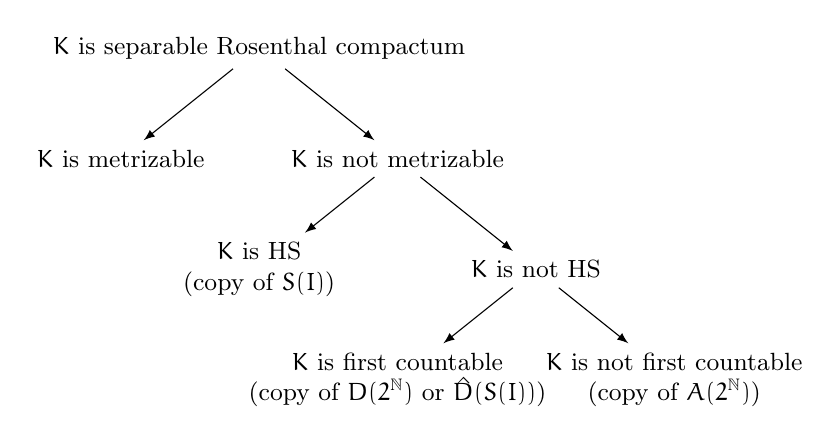
\begin{tikzpicture}[
  grow=down,
  sibling distance=10em,
  level distance=4em,
  edge from parent/.style={draw,-latex},
  every node/.style={font=\small,align=center}
  ]

\node {$K$ is separable Rosenthal compactum}
  child {node {$K$ is metrizable}
  }
  child {node {$K$ is not metrizable}
    child {node {$K$ is HS \\ (copy of $S(I)$)}}
    child {node {$K$ is not HS}
      child {node {$K$ is first countable \\ (copy of $D(2^\mathbb{N})$ or $\hat{D}(S(I))$)}}
      child {node {$K$ is not first countable \\ (copy of $A(2^\mathbb{N})$)}}
    }
  };

\end{tikzpicture}
\end{center}

Lastly, the definitions provided here for $NIP_i$ ($i=1,2,3$) are topological.

\begin{question}
    Is there a non-topological characterization for $NIP_i$, $i=1,2,3$?
\end{question}

\subsection{NIP and definability by universally measurable functions}

We now turn to the question: what happens when $\mathcal{P}$ is uncountable? Notice that the countability assumption is crucial in the proof of Theorem \ref{Generalized BFT} essentially because it makes $\mathbb{R}^\mathcal{P}$ a Polish space. For the uncountable case, we may lose Baire-1 definability so we shall replace $B_1(X)$ by a bigger class. Recall that the purpose of studying the class of Baire-1 functions is that a pointwise limit of continuous functions is not necessarily continuous. In \cite{BFT_1978_PCompactBaire}, J. Bourgain, D.H. Fremlin and M. Talagrand characterized the Non-Independence Property of a set of continuous functions with various notions of compactness in function spaces containing $C(X)$, such as $B_1(X)$. In this section we will replace $B_1(X)$ with the larger space $M_r(X)$ of universally measurable functions. The development of this section is based on Theorem 2F in \cite{BFT_1978_PCompactBaire}. We now give the relevant definitions. Readers with little familiarity with measure theory can review the appendix for standard definitions appearing in this subsection.

Given a Hausdorff space $X$ and a measurable space $(Y,\Sigma)$, we say that $f:X\rightarrow Y$ is \emph{universally measurable} (with respect to $\Sigma$) if $f^{-1}(E)$ is universally measurable for every $E\in\Sigma$, i.e., $f^{-1}(E)$ is $\mu$-measurable for every Radon probability measure $\mu$ on $X$. When $Y=\mathbb{R}$ we will always take $\Sigma=\mathcal{B}(\mathbb{R})$, the Borel $\sigma$-algebra of $\mathbb{R}$. In that case, a function $f:X\rightarrow\mathbb{R}$ is universally measurable if and only if $f^{-1}(U)$ is $\mu$-measurable for every Radon probability measure $\mu$ on $X$ and every open set $U\subseteq\mathbb{R}$. Following \cite{BFT_1978_PCompactBaire}, the collection of all universally measurable real-valued functions will be denoted by $M_r(X)$. In the context of deep computations, we will be interested in transition maps from a state space $L\subseteq \mathbb{R}^\mathcal{P}$ to itself. There are two natural $\sigma$-algebras one can consider in the product space $\mathbb{R}^\mathcal{P}$: the Borel $\sigma$-algebra, i.e., the $\sigma$-algebra generated by open sets in $\mathbb{R}^\mathcal{P}$; and the cylinder $\sigma$-algebra, i.e., the $\sigma$-algebra generated by Borel cylinder sets or equivalently basic open sets in $\mathbb{R}^\mathcal{P}$. Note that when $\mathcal{P}$ is countable, both $\sigma$-algebras coincide but in general the cylinder $\sigma$-algebra is strictly smaller. We will use the cylinder $\sigma$-algebra to define universally measurable maps $f:\mathbb{R}^\mathcal{P}\rightarrow\mathbb{R}^\mathcal{P}$. The reason for this choice is because of the following characterization:

\begin{lem}\label{lemma:coordinated_univ_meas}
    Let $X$ be a Hausdorff space and $Y=\prod_{i\in I}Y_i$ be any product of measurable spaces $(Y_i,\Sigma_i)$ for $i\in I$. Let $\Sigma_Y$ be the cylinder $\sigma$-algebra generated by the measurable spaces $(Y_i,\Sigma_i)$. Let $f:X\rightarrow Y$. The following are equivalent:
    \begin{itemize}
        \item [(i)] $f:X\rightarrow Y$ is universally measurable (with respect to $\Sigma_Y$).
        \item [(ii)] $\pi_i\circ f:X\rightarrow Y_i$ is universally measurable (with respect to $\Sigma_i$) for all $i\in I$.
    \end{itemize}
\end{lem}

\begin{proof}
    (i)$\Rightarrow$(ii) is clear since the projection maps $\pi_i$ are measurable and the composition of measurable functions is measurable. To prove (ii)$\Rightarrow$(i), suppose that $C=\prod_{i\in I}C_i$ is a measurable cylinder and let $J$ be the finite set of $i\in I$ such that $C_i\neq Y_i$. Then, $C=\bigcap_{i\in J}\pi_i^{-1}(C_i)$ so $f^{-1}(C)=\bigcap_{i\in J}(\pi_i\circ f)^{-1}(C_i)$ is a universally measurable set by assumption.
\end{proof}

The previous lemma says that a transition map is universally measurable if and only if it is universally measurable on all its features. In other words, we can check measurability of a transition just by checking measurability in all its features. We will denote by $M_r(X,\mathbb{R}^\mathcal{P})$ the collection of all universally measurable functions $f:X\rightarrow\mathbb{R}^\mathcal{P}$ (with respect to the cylinder $\sigma$-algebra), endowed with the topology of pointwise convergence.

\begin{defn}
    Let $(L,\mathcal P,\Gamma)$ be a CCS. We say that a transition $f:L\rightarrow L$ is \emph{universally measurable shard-definable} if and only if there exists $\tilde f:\mathcal{L}_{sh}\rightarrow \mathcal{L}_{sh}$ extending $f$ such that for every sizer $r_\bullet$ there is a sizer $s_\bullet$ such that the restriction $\tilde f|_{\mathcal{L}[r_{\bullet}]}:\mathcal{L}[r_\bullet]\rightarrow\mathcal{L}[s_\bullet]$ is universally measurable, i.e. $\pi_P\circ \tilde f|_{\mathcal{L}[r_{\bullet}]}:\mathcal{L}[r_\bullet]\rightarrow [-s_P,s_P]$ is $\mu$-measurable for every Radon probability measure $\mu$ on $\mathcal{L}[r_\bullet]$.
\end{defn}

We will need the following result about NIP and universally measurable functions:

\begin{thm}[Bourgain-Fremlin-Talagrand, Theorem 2F in \cite{BFT_1978_PCompactBaire}]\label{BFT-2F}
    Let $X$ be a Hausdorff space and $A\subseteq C(X)$ be pointwise bounded. The following are equivalent:
    \begin{itemize}
        \item [(i)] $\overline{A}\subseteq M_r(X)$.
        \item [(ii)] For every compact $K\subseteq X$, $A|_K$ has the NIP.
    \end{itemize}
\end{thm}

Theorem~\ref{BFT} immediately yields the following.

\begin{thm}
    Let $(L,\mathcal P,\Gamma)$ be a CCS satisfying the Extendibility Axiom. Let $R$ be an exhaustive collection of sizers. Let $\Delta\subseteq\Gamma$ be $R$-confined. If $\pi_P\circ\Delta|_{L[r_\bullet]}$ has the NIP for all $P\in\mathcal{P}$ and all $r_{\bullet}\in R$, then every deep computation is universally measurable shard-definable.
\end{thm}

\begin{proof}
    By the Extendibility Axiom, Theorem \ref{BFT} and lemma \ref{NIP and closure} we have that $\overline{\pi_P\circ\tilde\Delta|_{\mathcal{L}[r_\bullet]}}\subseteq M_r(\mathcal{L}[r_\bullet])$ for all $r_\bullet\in R$ and $P\in\mathcal{P}$. Let $f\in\overline{\Delta}$ be a deep computation. Write $f=\mathcal{U}\lim_i\gamma_i$ as an ultralimit of computations in $\Delta$. Define $\tilde f:=\mathcal{U}\lim_i\tilde\gamma_i$. Then, for all $r_\bullet\in R$ and $P\in\mathcal{P}$ $\pi_P \circ \tilde\gamma_i|_{\mathcal{L}[r_\bullet]}\in M_r(\mathcal{L}[r_\bullet])$ for all $i$ so $\pi_P \circ f|_{\mathcal{L}[r_\bullet]}\in \overline{\pi_P\circ\tilde\Delta|_{\mathcal{L}[r_\bullet]}}\subseteq M_r(\mathcal{L}[r_\bullet])$.
\end{proof}

\begin{question}
Under the same assumptions of the previous Theorem, suppose that every deep computation of $\Delta$ is universally measurable shard-definable. Must $\pi_P\circ\Delta|_{L[r_\bullet]}$ have the NIP for all $P\in\mathcal{P}$ and all $r_{\bullet}\in R$?
\end{question}

\subsection{Talagrand stability and definability by universally measurable functions}

There is another notion closely related to NIP, introduced by Talagrand in \cite{talagrand1984pettis} while studying Pettis integration. Suppose that $X$ is a compact Hausdorff space and $A\subseteq \mathbb{R}^X$. Let $\mu$ be a Radon probability measure on $X$. Given a $\mu$-measurable set $E\subseteq X$, a positive integer $k$ and real numbers $a<b$. we write:

$$D_k(A,E,a,b)=\bigcup_{f\in A}\{x\in E^{2k}:f(x_{2i})\leq a, \hspace{1mm} f(x_{2i+1})\geq b \hspace{1mm}{\text{ for all }i<k} \}$$

We say that $A$ is \emph{Talagrand $\mu$-stable} if and only if for every $\mu$-measurable set $E\subseteq X$ of positive measure and for every $a<b$ there is $k\geq 1$ such that $(\mu^{2k})^*(D_k(A,E,a,b))<(\mu(E))^{2k}$. Notice that we work with the outer measure because it is not necessarily true that the sets $D_k(A,E,a,b)$ are $\mu$-measurable. This is certainly the case when $A$ is a countable set of continuous (or $\mu$-measurable) functions. 

The following lemma establishes that Talagrand stability is a way to ensure that deep computations are definable by measurable functions. We include the proof for the reader's convenience.

\begin{lem}
    If $A$ is Talagrand $\mu$-stable, then $\overline{A}$ is also Talagrand $\mu$-stable and $\overline{A}\subseteq\mathcal{L}^0(X,\mu)$.
\end{lem}

\begin{proof}
    First, observe that a subset of a $\mu$-stable set is $\mu$-stable. To show that $\overline{A}$ is $\mu$-stable, observe that $D_k(\overline{A},E,a,b)\subseteq D_k(A,E,a',b')$ where $a<a'<b'<b$ and $E$ is a $\mu$-measurable set with positive measure. It suffices to show that $\overline{A}\subseteq \mathcal{L}^0(X,\mu)$. Suppose that there exists $f\in\overline{A}$ such that $f\notin \mathcal{L}^0(X,\mu)$. By a characterization of measurable functions (see 413G in \cite{fremlin2003vol4}), there exists a $\mu$-measurable set $E$ of positive measure and $a<b$ such that $\mu^*(P)=\mu^*(Q)=\mu(E)$ where $P=\{x\in E: f(x)\leq a\}$ and $Q=\{x\in E: f(x)\geq b\}$. Then, for any $k\geq 1$: $(P\times Q)^k\subseteq D_k(\{f\},E,a,b)$ so $(\mu^{2k})^*(D_k(\{f\},E,a,b))=(\mu^*(P)\mu^*(Q))^k=(\mu(E))^{2k}$. Thus, $\{f\}$ is not $\mu$-stable, but we argued before that a subset of a $\mu$-stable set must be $\mu$-stable.
\end{proof}

We say that $A$ is \emph{universally Talagrand stable} if $A$ is Talagrand $\mu$-stable for every Radon probability measure $\mu$ on $X$. A similar argument as before, yields the following:

\begin{thm}
    Let $(L,\mathcal P,\Gamma)$ be a CCS satisfying the Extendibility Axiom. If $\pi_P\circ\Delta|_{L[r_\bullet]}$ is universally Talagrand stable for all $P\in\mathcal{P}$ and all sizers $r_{\bullet}$, then every deep computation is universally measurable sh-definable.
\end{thm}

It is then natural to ask: what is the relationship between Talagrand stability and the NIP? We know that Theorem \ref{BFT-2F} and Fremlin's Dichotomy (463K in \cite{fremlin2003vol4}) imply:

\begin{lem}
    Let $X$ be a compact Hausdorff space and $A\subseteq C(X)$ be pointwise bounded. If $A$ is universally Talagrand stable, then $A$ has the NIP.
\end{lem}

\begin{question}
    Is the converse true?
\end{question}

There is a delicate point in this question, as it may be sensitive to set-theoretic axioms (even assuming countability of $A$).

\begin{thm}[Talagrand, Theorem 9-3-1(a) in \cite{talagrand1984pettis}]
    Let $X$ be a compact Hausdorff space and $A\subseteq M_r(X)$ be countable and pointwise bounded. Assume that $[0,1]$ is not the union of $<\mathfrak{c}$ closed measure zero sets. If $A$ has the NIP, then $A$ is universally Talagrand stable.
\end{thm}

\begin{thm}[Fremlin, Shelah, \cite{fremlin1993pointwise}]
    It is consistent that there exists a countable pointwise bounded set of Lebesgue measurable functions with the NIP which is not Talagrand stable with respect to Lebesgue measure.
\end{thm}

\section*{Appendix: Measure Theory}

Given a set $X$, a collection $\Sigma$ of subsets of $X$ is called a \emph{$\sigma$-algebra} if $\Sigma$ contains $X$ and is closed under complements and countable unions. Hence, for example, a $\sigma$-algebra is also closed under countable intersections. Intuitively, a $\sigma$-algebra is a collection of sets in which we can define a $\sigma$-additive measure. We call sets in a $\sigma$-algebra $\Sigma$ \emph{measurable sets} and the pair $(X,\Sigma)$ a measurable space. If $X$ is a topological space, there is a natural $\sigma$-algebra of subsets of $X$, namely the \emph{Borel $\sigma$-algebra} $\mathcal{B}(X)$, i.e., the smallest $\sigma$-algebra containing all open subsets of $X$. Given a measurable space $(X,\Sigma)$, a \emph{$\sigma$-additive measure} is a non-negative function $\mu:\Sigma\rightarrow\mathbb{R}$ with the property that $\mu(\emptyset)=0$ and $\mu(\bigcup_{n=0}^\infty A_n)=\sum_{n=0}^\infty\mu(A_n)$ whenever $\{A_n:n\in\mathbb{N}\}\subseteq\Sigma$ is pairwise disjoint. We call $(X,\Sigma,\mu)$ a \emph{measure space}. A $\sigma$-additive measure is called a \emph{probability measure} if $\mu(X)=1$. A measure $\mu$ is \emph{complete} if for every $A\subseteq B\in\Sigma$, $\mu(B)=0$ implies $A\in\Sigma$. In words, subsets of measure-zero sets are always measurable (and hence, by the monotonicity of $\mu$, have measure zero as well).

A special example of the preceding concepts is that of a \emph{Radon measure}. If $X$ is a Hausdorff topological space, then a measure $\mu$ on the Borel sets of $X$ is called a \emph{Radon measure} if
\begin{itemize}
    \item for every open set $U$, $\mu(U)$ is the supremum of $\mu(K)$ over all compact $K\subseteq U$, that is, the measure of open sets may be approximated via compact sets; and
    \item every point of $X$ has a neighborhood $U\ni x$ for which $\mu(U)$ is finite.
\end{itemize}

Perhaps the most famous example of a Radon measure on $\mathbb R$ is the Lebesgue measure of Borel sets. If $X$ is finite, $\mu(A):=|A|$ (the cardinality of $A$) defined a Radon measure on $X$.

While not immediately obvious, sets can be measurable according to one measure, but non-measurable according to another. Given a measure space $(X,\Sigma,\mu)$ we say that a set $E\subseteq X$ is \emph{$\mu$-measurable} if there are $A,B\in \Sigma$ such that $A\subseteq E\subseteq B$ and $\mu(B\backslash A)=0$. The set of all $\mu$-measurable sets is a $\sigma$-algebra containing $\Sigma$ and it is denoted by $\Sigma_\mu$. A set $E\subseteq X$ is \emph{universally measurable} if it is $\mu$-measurable for every Radon probability measure on $X$. It follows that Borel sets are universally measurable.

Recall that if $\{X_i:i\in I\}$ is a collection of topological spaces indexed by some set $I$, then the product space $X:=\prod_{i\in I}X_i$ is endowed with the topology generated by \emph{cylinders}, that is, sets of the form $\prod_{i\in I} U_i$ where each $U_i$ is open in $X_i$, and $U_i=X_i$ except for finitely many indices $i\in I$. If each space is measurable, say we pair $X_i$ with a $\sigma$-algebra $\Sigma_i$, then there are multiple ways to interpret the product space $X$ as a measurable space, but the interpretation we care about in this paper is the so called \emph{cylinder $\sigma$-algebra}, as used in Lemma~\ref{lemma:coordinated_univ_meas}. Namely, let $\Sigma$ be the $\sigma$-algebra generated by sets of the form $$\prod_{i\in I}C_i,\quad C_i\in\Sigma_i,\ C_i=X_i\ \text{for all but finitely many }i\in I.$$

We remark that when $I$ is uncountable and $\Sigma_i=\mathcal B(X_i)$ for all $i\in I$, then $\Sigma$ is, in general, strictly \textbf{smaller} than $\mathcal B(X)$.

%%%%%%%%%%%%%%%%%%%%%%%%%%%%%%%%%%%%%%%%%%%%%%%%%%%%%%%%%%%%%%%%%%%%%%%%%%

%Proof below was simplified by the previous

%\begin{thm}
    %Let $X$ be a Polish space, $\mathcal{P}$ be a countable set and $Y=\mathbb R^\mathcal P$. Let $A\subseteq C_p(X,Y)$ be a pointwise bounded set (i.e. for all $x\in X$, there is a sizer $r_{\bullet}^x=\{r_P^x\}_{P\in\mathcal{P}}$ such that for all $f\in A$ and $P\in\mathcal P$, $\pi_P\circ f(x)\in[-r_P^x,r_P^x]$). The following are equivalent:

    %\begin{itemize}
        %\item [(i)] For every compact $K\subseteq X$, $A|_K$ is relatively compact in $B_1(K,Y)$.
        %\item [(ii)] For every compact $K\subseteq X$, $\overline{A|_K}\subseteq B_1(X,Y)$.
        %\item [(iii)] For every compact $K\subseteq X$, for every $P\in\mathcal P$, $\{f_n\}_n\subseteq A$ and reals $\alpha<\beta$, there is $I\subseteq\mathbb N$ such that for any $p\in\mathcal P'$,
    %$$
    %\bigcap_{n\in I}(p\circ f)^{-1}(-\infty,\alpha]\cap\bigcap_{n\notin I}(p\circ f)^{-1}[\beta,\infty)\cap K=\emptyset.
    %$$
        %\item [(iv)] For any relatively compact $L$, for any finite $\mathcal P'\subseteq\mathcal P$, $\{f_n\}_n\subseteq A$ and reals $\alpha<\beta$, there are disjoint finite sets $F,G\subseteq\mathbb N$ such that for any $p\in\mathcal P'$,$$\bigcap_{n\in F}(p\circ f)^{-1}(-\infty,\alpha]\cap\bigcap_{n\in G}(p\circ f)^{-1}[\beta,\infty)\cap L=\emptyset.$$
    %\end{itemize}
%\end{thm}



%\subsection{Proof of the conjecture}

%$\boxed{1\implies 2}$

%Denote $F:=A|_K$ and suppose that $f\in\overline F\setminus B_1(X,Y)$. Lemma 1 implies that $\hat f\notin B_1(\mathcal P\times X)$. Since $\mathcal P\times X$ is a Polish space, we apply Fact~\ref{baire} to find reals $\alpha<\beta$ and countable sets $D_0,D_1\subseteq\mathcal P\times X$ with $\overline{D_0}=\overline{D_1}$, $D_0\subseteq\hat f^{-1}(-\infty,\alpha]$ and $D_1\subseteq\hat f^{-1}[\beta,\infty)$.

%For each $p\in\mathcal P$ and $i<2$, let $D_i^p:=\{x\in X:(p,x)\in D_i\}$ and consider $D=\bigcup_{p\in\mathcal P}(D_0^p\cup D_1^p)$. Since $D$ is countable, enumerate it in order type $\omega$, $D=\{x_i:i<\omega\}$.

%This is Stevo's diagonal argument. For each $n\geq1$, find $f_n\in F$ such that the distance between $f(x_i)$ and $f_n(x_i)$ is less than $1/n$ for all $i\leq n$. Then, for all fixed $i<\omega$, if $n\geq i$, then for every fixed $x\in D$, $\lim_{n\to\infty}f_n(x)=f(x)$.

%$F$ is not just relatively compact, but relatively countably compact. Thus, let $g\in B_1(X,Y)$ be an accumulation point of $\{f_n\}_n$. It is clear that $f_D=g|_D$, since $g=\lim_{k\to\infty}f_{n_k}$, and thus for all $x\in D$, $g(x)=\lim_{k\to\infty}f_{n_k}(x)=\lim_{n\to\infty}f_n(x)=f(x)$.

%It follows that $D_0\subseteq\hat g^{-1}(-\infty,\alpha]$ and $D_1\subseteq\hat g^{-1}[\beta,\infty)$. Let $E:=\overline{D_0}=\overline{D_1}$. By Fact~\ref{baire}, $\hat g|_E$ must have a point of continuity $x\in E$. Let $\varepsilon:=\frac{\beta-\alpha}2>0$ and find $\delta>0$ such that $d(x,y)<\delta$ implies $|\hat g(x)-\hat g(y)|<\varepsilon$. By density arguments, find for each $i$ an $x_i\in D_i$, with $d(x,x_i)<\delta$. But then, the triangle inequality and the choice of $\alpha,\beta$ give $\beta-\alpha\leq|\hat g(x_0)-\hat g(x_1)|<\beta-\alpha$, a contradiction.

%$\boxed{2\implies 3}$

%To prove the remaining implication we need:

%\begin{lem}
    %$\overline{\hat A|_K}\setminus B_1(\mathcal P\times X)\neq\emptyset$ implies that $\overline{A|_K}\setminus B_1(X,Y)\neq\emptyset$.
%\end{lem}

%%%%%%%%%%%%%%%%%%%%%%%%%%%%%%%%%%%%%%%%%%%%%%%%%%%%%%%%%%%%%%%%%

%\begin{thebibliography}{9}

\bibliographystyle{alpha}
\nocite{*}
\bibliography{bib}

%\end{thebibliography}
\end{document}